% Use only LaTeX2e, calling the article.cls class and 12-point type.

\documentclass[12pt]{article}
%\documentclass[twoside,a4,12pt]{article}

\usepackage{scicite}

\usepackage{times}

\usepackage{subfigure}
\usepackage{amsmath, amsthm, amssymb}
\usepackage{epsf,graphicx}
\usepackage{latexsym,amssymb}
\usepackage{setspace,cite}
\usepackage[pagebackref=true,breaklinks=true,letterpaper=true,colorlinks,bookmarks=false]{hyperref}
\usepackage[french,british]{babel}
\usepackage{array}
\usepackage{multirow}
\usepackage{url}
%\documentclass{article}
\usepackage{subfigure}
\usepackage{amsmath}



% The following parameters seem to provide a reasonable page setup.

\topmargin 0.0cm
\oddsidemargin 0.2cm
\textwidth 16cm 
\textheight 21cm
\footskip 1.0cm


%The next command sets up an environment for the abstract to your paper.

\newenvironment{sciabstract}{%
\begin{quote} \bf}
{\end{quote}}


% If your reference list includes text notes as well as references,
% include the following line; otherwise, comment it out.

\renewcommand\refname{References and Notes}

% The following lines set up an environment for the last note in the
% reference list, which commonly includes acknowledgments of funding,
% help, etc.  It's intended for users of BibTeX or the {thebibliography}
% environment.  Users who are hand-coding their references at the end
% using a list environment such as {enumerate} can simply add another
% item at the end, and it will be numbered automatically.

\newcounter{lastnote}
\newenvironment{scilastnote}{%
\setcounter{lastnote}{\value{enumiv}}%
\addtocounter{lastnote}{+1}%
\begin{list}%
{\arabic{lastnote}.}
{\setlength{\leftmargin}{.22in}}
{\setlength{\labelsep}{.5em}}}
{\end{list}}


% Include your paper's title here

\title{Intrinsic Camera Calibration Equipped with Scheimpflug Optical Device} 


% Place the author information here.  Please hand-code the contact
% information and notecalls; do *not* use \footnote commands.  Let the
% author contact information appear immediately below the author names
% as shown.  We would also prefer that you don't change the type-size
% settings shown here.

\author
%\ast
{Peter Fasogbon$^{1,2}$, Luc Duvieubourg$^{1}$, Pierre-Antoine Lacaze$^{2}$, Ludovic Macaire$^{1}$\\
\\
\normalsize{$^{1}$Laboratoire Lagis, Universit\'{e} of Lille1, UMR CNRS 8219}\\
\normalsize{Cit\'{e} Scientifique - Bat P2 - 59655 Villeneuve d'Ascq Cedex}\\
\normalsize{$^{2}$SNCF Direction de l'Ingi\'{e}nerie, ---, Plaine Saint Senis, FRANCE}\\
\\
\normalsize{$^\ast$ E-mail:  faspetpeak@yahoo.com}
}

% Include the date command, but leave its argument blank.

\date{}



%%%%%%%%%%%%%%%%% END OF PREAMBLE %%%%%%%%%%%%%%%%



\begin{document} 

% Double-space the manuscript.

\baselineskip24pt

% Make the title.

\maketitle 




\section*{Introduction}


For many cameras to be in perfect focus, an object must be placed in a plane surface that is parallel to the image plane. However, acquiring an image at sharp focus can be very difficult when the surface of interest is located in an oblique plane to the optical axis (i.e. object plane not parallel to the image plane). It is the case when the camera observes the facade of a tall building or a decorative cobblestone pathway. The camera can be aimed upward at an angle which makes it difficult to bring the complete surface of interest in focus.  Therefore, for a certain oblique plane to be in focus, the imaging set-up must obey "Scheimpflug's principle" \cite{Astarita:2012}. 

We have used Scheimpflug technique so that the sharp camera's field of view is as wide as possible. This system is specifically designed for 3D dimensional measurement under Scheimpflug condition. So, we have to perform an intrinsic camera calibration in order to extract accurate 3D measures from 2D images. Intrinsic calibration has been extensively studied  in computer vision and photogrammetry community and various techniques have been proposed over the past few years \cite{Salvi:2000}.

However, classical camera calibration techniques based on pinhole model cannot be used directly with Scheimpflug system set-up \cite{Prasad95}. Therefore, we describe the Scheimpflug set-up and propose an image formation model when the camera is equipped with a Scheimpflug lens. Then, we detail the intrinsic calibration method that is adapted to the Scheimpflug set-up. Finally, first experimental results are presented to assess the performance of our proposed method. 


\section{Scheimpflug image formation model}

%The Scheimpflug principle calls for the oblique plane containing the observed surfaces, the image plane, and the lens plane to intersect in a common line.



For classical pin-hole model, the image plane is usually parallel to the lens plane, so that it is perpendicular to the optical axis.  However, for Scheimpflug set-up, the image plane is tilted at a given angle ${\bf{\theta}}$ around the optical center (see  Figure \ref{fig:scheimpflug2}). This adjustment  ensures that the image plane, the lens plane and the object plane intersect at a line parallel to $X_c$ axis, denoted as  "scheimpflug line" and represented as a point in Figure \ref{fig:scheimpflug2}. In that case, the field of view according the oblique plane is larger than for classical lens.  

\begin{figure}[htb]
	\centering
	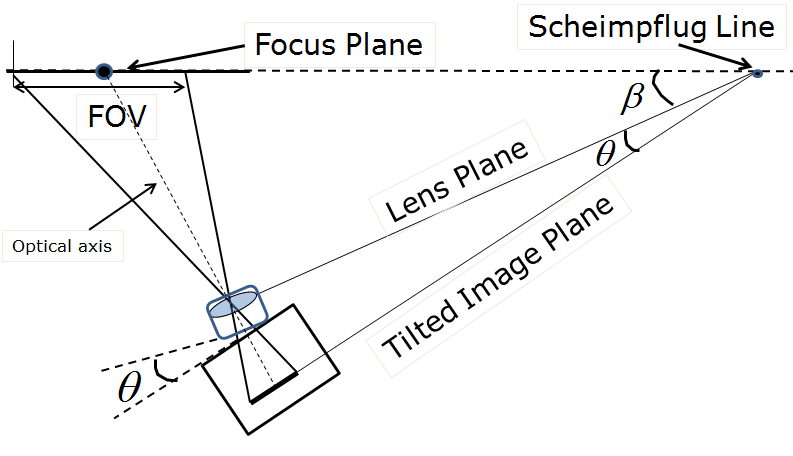
\includegraphics[height=6cm, width=10cm]{figures/scheimpflug1.png}
	\caption {Scheimpflug System Set-up}

	\label{fig:scheimpflug2}
\end{figure}




%\begin{figure}[htb]
%%\begin{centering}
%	\subfigure[]{\includegraphics[height=5cm, width=5cm]{figures/scheimpflug2.jpg}}
%%\hfill
%\subfigure[]{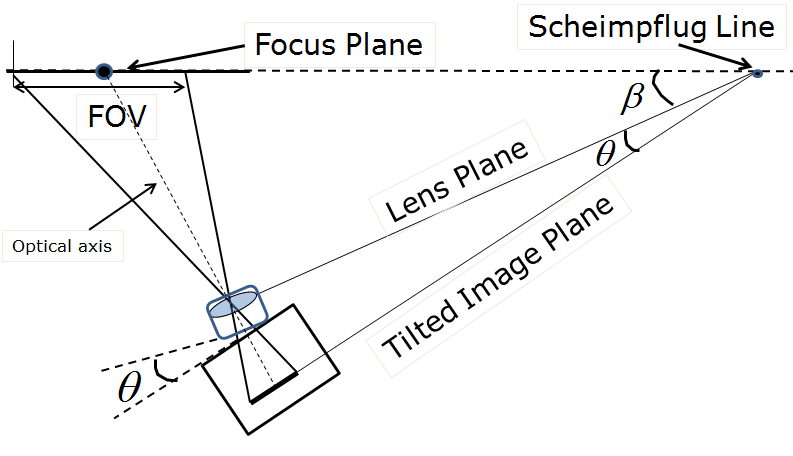
\includegraphics[height=4.4cm, width=7cm]{figures/scheimpflug1.jpg}}
%%\hfill
%	%\subfigure[Not mine]{\includegraphics[height=4cm, width=5cm]{figures/wirewearhof.jpg}}
%	\caption{Classical System Set-up and Scheimpflug}
%	\label{fig:scheimpflug2}
%%\end{centering}
%\end{figure}



A point $P$ along the object focus plane (see Figure \ref{fig:scheimpflug3}) is projected into the point $p_t$ in the tilted image plane. Let us denote $d_{i}= \|\vec {O_c~p_t^a}\|$ and $d_{o}= \|\vec {O_c~P^a}\|$ the image and object distances from the center $O_c$ of the lens along the optical axis, where $p_t^a$ and $P^a$ are the projections of $p_t$ and $P$ to the optical axis.  The thin lens equations still hold for Scheimpflug set-up so that $\frac{1}{f}=\frac{1}{do}+\frac{1}{di}$, where $f$ is the focal length. This is possible for any points along the object focus plane that are projected to the tilted image plane.  When the object of interest is located at an angle $\beta$ to the lens plane, the lens plane is tilted with respect to the Scheimpflug angle $\theta$ so that the focus plane is brought to the object location. \\


\begin{figure}[htb]
	\centering
	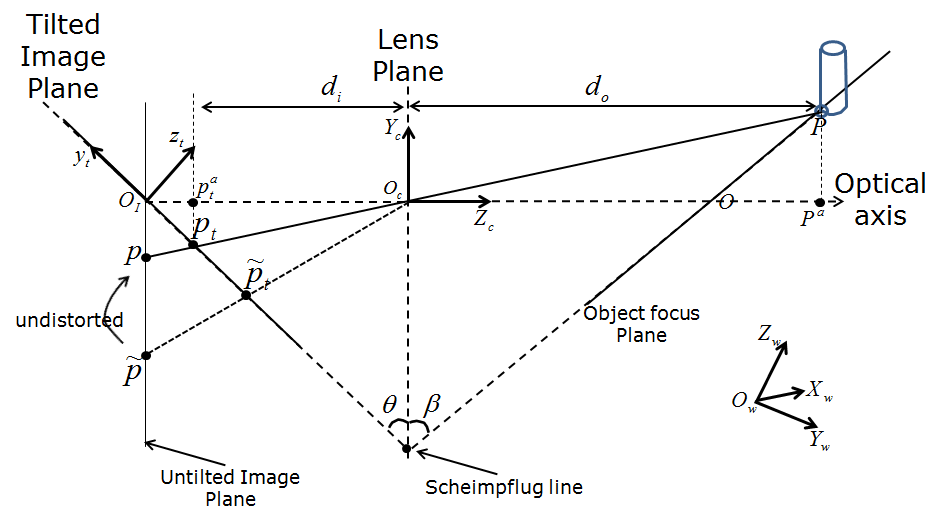
\includegraphics[height=6cm, width=12cm]{figures/scheimimg1.png}
	\caption {Scheimpflug camera model.}
	\label{fig:scheimpflug3}
\end{figure}

%We distinguish the following coordinate systems:
%\begin{itemize}
%\item  The world coordinate system $(O_w[X_{w},Y_{w},Z_{w}])$,
%\item  The camera/lens coordinate system $(O_c[X_{c},Y_{c},Z_{c}])$,
%\item  The untilted image coordinate system,$(O_I[x,y,z])_I$, where $z=0$ for each point on the untilted image plane,
%\item  The tilted image coordinate system $(O_I[x_{t},y_{t},z_{t}])_t$, where $z_t=0$ for each point on the tilted image plane, 
%\item  The untilted pixel coordinate system $(O_p[u,v])$, 
%\item  The tilted pixel coordinate system, $(O_p[u_t,v_t])$
%\end{itemize}


%The origins of the tilted and the perpendicular plane are the same, as the perpendicular plane can be arbitrarily placed.





%, distorted point $p_d = ({x},{y})^T$, undistorted point $p_u = (x,y)^T$ , with a distorted point $p_t = ({x_{t}},{y_{t}})^T$ , with a distorted pixel $p_d = ({u},{v})^T$, undistorted $p_u = (u,v)^T$, distorted tilted $p_t = ({u_t},{v_t})^T$, and undistorted tilted $p_t = (u_t,v_t)^T$.

In order to determine the 3D coordinates of world point $P$ from its projected point $p_t$ in the tilted image plane, we need to calibrate the used camera. Therefore, we have proposed a Scheimpflug calibration method based on pin-hole model assumptions. 


%\subsection{Zhang Calibration}

%We can now derive the scheimpflug camera model from the pinhole one. 

\subsection{Image formation for Scheimpflug angle}


%
%Using homogeneous coordinate representation and assuming no optical distortion, an object point $P (X_{w},Y_{w},Z_{w},1) $ is first projected to the point $p (x,y,0,1)_I $ in the untilted image plane as
%
%\begin{equation}  
%\lambda~p = \mathcal{K}_f \begin{bmatrix}
%\mathcal{R} \mid \mathcal{T}\\
%\end{bmatrix}  P
%\label{eqn:projm20}
%\end{equation}
%
%where intrinsic parameter $\mathcal{K}_f =\begin{bmatrix}
%f&0&0\\
%0&f&0\\
%0&0&1\\
%\end{bmatrix}$ , and extrinsic $\mathcal{R}$, and $\mathcal{T}$ [{\it 1}].\\
%
%In order to project the point $P$ onto the untilted image plane, we first need to simplify the optical distortion. If we consider radial distortions only, we can express the coordinates of the undistorted point $p (x,y,0)_I$ from the coordinates of the distorted one ${p}({x},{y},0)_I$ in the same untilted plane as,
%
%\begin{equation}
%\begin{split}
%{p}({x},{y},0)_I^T= p(x,y,0)_I^T + \delta_{(x,y,0)}  \\
%where~\delta_{(x,y,0)} =(\delta_x,\delta_y,0)
%\label{fig:dist2a}
%\end{split}
%\end{equation}
%
%%where $k_{i}'s$ are the radial distortion coefficients and $r=\sqrt{{x}^2+{y}^2}$ is the radial distance from the centre of the lens. Note that we can't easily express $p_d({x}, {y})$ as a function of $p_u(x,y)$, but has been shown it can be approximated[link]. \\
%
%
%Now, let us model image formation on the tilted image plane. Assuming optical distortion, a ray originating from the the optical center $O_c$ of the camera intersects the tilted plane at ${p_t}({x_t},  {y_t},0)_t$ and the untilted at ${p}({x},{y},0)_I$ respectively. Without abuse of notations, we represent a distorted point ${p_t}({x_t},{y_t},0)_t$ in the tilted plane as  ${p}_{c}^t({X_c},{Y_c},{Z_c})$ in the camera coordinate system, likewise point ${p}({x},{y},0)_I$ in the untilted image plane as ${p_{c}} ({X_c},{Y_c},{Z_c}=f)$. Therefore, the camera coordinate points ${p_{c}} ({X_c},{Y_c},{Z_c}=f)$ can be related to the untilted coordinate points ${p}({x},{y},0)_I$ as,
%
%\begin{equation}
%\begin{split}
%{X_c}= {x} \\
%{Y_c}= {y} \\
%{Z_c}= f \\
%\end{split}
%\end{equation}
%
%We have formulated a projective transformation $\mathcal{K}_{c}^t$ under Scheimpflug model. We first applied this matrix $\mathcal{K}_{c}^t$ of the distorted point ${p_{c}}({X_c},{Y_c},f)$ to ${p}_{c}^t({X_c},{Y_c},{Z_c})$ as shown below: %(see appendix \ref{subsect:proof1} for $\mathcal{K}_{c}^t$ matrix formulation): 
%
%
%\begin{equation}  
%{p}_{c}^t=\mathcal{K}_{c}^t {p_{c}},  ~ \text{where}~\mathcal{K}_{c}^t=\begin{bmatrix}
%f & 0 & 0\\
%0 & f & 0 \\
%0 & 0 & f \\
%0 & -tan~\theta & 1 
%\end{bmatrix} 
%\label{eqn:Ad20}
%\end{equation}
%
%
%%\begin{equation}  
%%\mathcal{K}_{c}^t=\begin{bmatrix}
%%f & 0 & 0\\
%%0 & f & 0 \\
%%0 & 0 & f \\
%%0 & -tan~\theta & 1 
%%\end{bmatrix} 
%%\label{eqn:Ad}
%%\end{equation}
%
%
%
%%We apply this matrix of the distorted point  $p_d = [{x},{y},{z},1]$ to  $p_t = [{x_t},{y_t},{z_t},1]$ in the tilted image plane (see the appendix for the ${\bf{K_{pt}}}$ matrix formulation).  We are actually looking for the position of point $p_t$ in lens coordinate system, thanks to this matrix. \\
%
%Then we express the camera coordinates of the point ${p}_{c}^t({X_c},{Y_c},{Z_c})$   in the tilted image plane (i.e to have ${p_t} ({x_{t}},{y_{t}},0)_t$). This is done by applying rotation $\mathcal{R}_{s}$ with respect to the X-axis parametrised by angle $\theta$, preceded by a translation vector $\mathcal{T}_{s}$  (from $O_c$ to $O_I$). Finally we have our  $\mathcal{K}_{s}$ matrix as below,
%
%
%\begin{equation}  
%\begin{split}  
%\mathcal{K}_{s} = \begin{bmatrix}
%\mathcal{R}_{s} & \mathcal{T}_{s}\\
%0^{T} & 1\\
%\end{bmatrix}  =\begin{bmatrix}
%1& 0 & 0&0 \\
%0 & cos~\theta  & sin~\theta &0 \\
%0 & -sin~\theta & cos~\theta&0\\
%0 & 0 & 0 & 1
%\end{bmatrix} \begin{bmatrix}
%1 & 0 & 0&0 \\
%0 & 1 & 0&0 \\
%0 & 0 & 1&-f \\
%0 & 0 & 0 & 1 
%\end{bmatrix} \\
%\mathcal{K}_s=\begin{bmatrix}
%1& 0 & 0&0 \\
%0 & cos~\theta  & sin~\theta &-f~sin~\theta \\
%0 & -sin~\theta & cos~\theta&-f~cos~\theta\\
%0 & 0 & 0 & 1
%\end{bmatrix}
%\end{split}  
%\label{eqn:Ad1}
%\end{equation}  
%
%
%Note that the two steps described earlier complete the scheimpflug image formation ("Intrinsic formation"). Hence, the point ${p_t}({x_t},{y_t},0)_t$ on the tilted image plane is deduced from ${p_{c}} ({X_c},{Y_c},f)$ in the camera coordinate system as below
%
%\begin{equation}  
%\lambda {p_t} = \mathcal{K}_{s}\mathcal{K}_{c}^t{p_{c}}
%\label{eqn:sch1}
%\end{equation}
%
%
%A final conversion in pixel coordinates is effected with $\mathcal{K}_{b}$ matrix where $s_x,s_y,s_z$ are the pixel sizes and $(u_{0},v_{0})$ are the principal point coordinates in pixel unit. The pixel size $s_z$ can be changed to one since it will finally be cancelled out in the equation later on.
%
%\begin{equation}  
%\mathcal{K}_b=\begin{bmatrix}
%1/s_x & 0 & 0&u_{0} \\
%0 & 1/s_y & 0& v_{0} \\
%0 & 0 & 1/s_z&0 \\
%0& 0 & 0 & 1 
%\end{bmatrix} 
%\label{eqn:Ab3}
%\end{equation}
%
%Here is the full equation that that relates points ${p_{c}} ({X_c},{Y_c},f)$ to ${p_t}({u_t},{v_t})$ in pixel coordinates:
%
%\begin{equation}  
%\lambda {p_t} = \mathcal{K}_{b} \mathcal{K}_{s}\mathcal{K}_{c}^t{p_{c}}\\
%\label{eqn:sch1}
%\end{equation}
%
%\begin{equation}  
%\lambda  \begin{bmatrix}
%{u_t}\\
%{v_t}\\
%0\\
%1\\
%\end{bmatrix} =\begin{bmatrix}
%1/s_x & 0 & 0&u_{0} \\
%0 & 1/s_y & 0& v_{0} \\
%0 & 0 & 1&0 \\
%0& 0 & 0 & 1 
%\end{bmatrix} \begin{bmatrix}
%1& 0 & 0&0 \\
%0 & cos~\theta & sin~\theta  & -f~sin~\theta \\
%0 & -sin~\theta & cos~\theta&-f~cos~\theta\\
%0 & 0 & 0 & 1
%\end{bmatrix} \begin{bmatrix}
%f & 0 & 0\\
%0 & f & 0 \\
%0 & 0 & f\\
%0 & -tan~\theta & 1 
%\end{bmatrix} \begin{bmatrix}
%{X_c}\\
%{Y_c}\\
%f\\
%\end{bmatrix}
%\label{eqn:sch28}
%\end{equation}
%


The spatial pixel coordinates $p_t(u_t,v_t)$ in the tilted image plane is deduced from the coordinates $P(X,Y,Z)$ of the point in the word coordinate system under pin-hole model assumption, thanks to 3 successive equations. 
 Equation (\ref{eqn:scha}) first converts the world coordinates $P(X,Y,Z)$ of a scene point into camera coordinate system $P(X_c,Y_c,Z_c)$ with extrinsic parameters, i.e. the rotation $\mathcal{R}$ and translation $\mathcal{T}$ parameters. To model the projection to the tilted image plane, we propose to consider first the virtual image plane that is perpendicular to the optical axis and is called hereafter untilted image plane.
 Equation  (\ref{eqn:schb})  computes the coordinates $(x,y)$ of the projected point into the virtual untilted image plane thanks to the focal distance $f$. Equation (\ref{eqn:schc}) transforms the spatial coordinates $(x,y)$ in the untilted image plane to pixel coordinates $(u_t,v_t)$ in the tilted image plane, thanks to the intrinsic parameters to be estimated, i.e. the Scheimpflug angle $\theta$, the focal lens  $f$,  the pixel sizes $s_x$, $s_y$, and the image center pixel coordinates $u_0$, and $v_0$. 
 

\begin{equation}  
%\begin{split}
\begin{bmatrix}
X_c\\
Y_c\\
Z_c\\
\end{bmatrix} =
 \begin{bmatrix}
\mathcal{R} \mid \mathcal{T}\\
\end{bmatrix}
%\begin{bmatrix}
%r_{11}& r_{12} & r_{13}&t_x \\
%r_{21}& r_{22} & r_{23}&t_y \\
%r_{31}& r_{32} & r_{33}&t_z
%\end{bmatrix}  
\begin{bmatrix}
X\\
Y\\
Z\\
1
\end{bmatrix}\\
\label{eqn:scha}
\end{equation}

\begin{equation}  
\lambda\begin{bmatrix}
x\\
y\\
1\\
\end{bmatrix} =\begin{bmatrix}
f& 0 & 0 \\
0& f & 0 \\
0& 0 & 1
\end{bmatrix}  \begin{bmatrix}
X_c\\
Y_c\\
Z_c
\end{bmatrix}\\
\label{eqn:schb}
\end{equation}

\begin{equation}  
\lambda\begin{bmatrix}
u_t\\
v_t\\
1\\
\end{bmatrix} =\begin{bmatrix}
1/s_x & 0 & 0&u_{0} \\
0 & 1/s_y & 0& v_{0} \\
0 & 0 & 0&0 \\
0& 0 & 0 & 1 
\end{bmatrix}\begin{bmatrix}
1& 0 & 0&0 \\
0 & cos~\theta & sin~\theta  & -f~sin~\theta \\
0 & -sin~\theta & cos~\theta&-f~cos~\theta\\
0 & 0 & 0 & 1
\end{bmatrix} \begin{bmatrix}
f & 0 & 0\\
0 & f & 0 \\
0 & 0 & f\\
0 & -tan~\theta & 1 
\end{bmatrix} \begin{bmatrix}
x\\
y\\
f\\
\end{bmatrix}
%\end{split}
\label{eqn:schc}
\end{equation}



%However, we need to give initial values for , and $s_y$ in order to use the above equation. These values should be very close to the true ones to ensure fast  convergence of the subsequent minimization steps. We can use the values given by the manufacturer for $f$, the pixel sizes $s_x$, $s_y$, and the image center $u_0$, and $v_0$ respectively.


\section{Intrinsic calibration steps}

To estimate the intrinsic parameters and especially the Scheimpflug angle $\theta$, we adapt the classical  calibration technique proposed by Zhang et al. \cite{Zhang:2000:FN} that uses a target plane composed of $n$ feature points and placed in the scene according to $m$ poses.  Each point of the calibration target in the world coordinate system $P^{(i,j)} ({X}^{(i,j)}, {Y}^{(i,j)} {Z}^{(i,j)})$ ($i=1,..,n$, $j=1,..,m$) is matched to its corresponding pixel ${p}_t^{(i,j)}({u}_t^{(i,j)},{v}_t^{(i,j)})$ in the tilted image plane.  The Scheimpflug camera calibration that analyses the given pixels ${p}_t^{(i,j)}$ in the tilted image plane, is decomposed into three successive steps as described below.

\subsection{Projection to the Untilted Image Plane}
As a result of distortion introduced by tilt effect, we thereby propose to perform the calibration procedure on the untilted "virtual" image plane. The given pixels ${p}_t^{(i,j)}({u}_t^{(i,j)},{v}_t^{(i,j)})$ in the tilted image plane are transformed into  points ${p}_c^{(i,j)} ({X_c}^{(i,j)},{Y_c}^{(i,j)},f)$ in the untilted image plane, and expressed in the camera coordinate system according to equations (\ref{eqn:scha})-(\ref{eqn:schc}).  For this purpose, we need to give initial values of  $\theta$, $f$,  $s_x$, $s_y$,  $u_0$, and $v_0$ (given by the manufacturer) in order to apply the above equations. These values should be very close to the true ones to ensure fast convergence of the following minimization steps. 


\subsection{Target-image plane homography estimation}
 The projective transformation between each pose of the calibration target plane and the untilted image plane is an homography. To estimate it, we need feature points $P^{(i,j)} ({X}^{(i,j)}, {Y}^{(i,j)}, {Z}^{(i,j)})$ of the calibration target, and their corresponding pixels ${p}^{(i,j)} ({u}^{(i,j)},{v}^{(i,j)})$ on the untilted image plane. We can then apply the normalized Direct Linear Transformation algorithm (DLT) method  to extract the homography matrix $\mathcal{H}_{(j)}$ at each pose $j$ of the calibration target \cite{Hartley:2003:MVG}.  \\
%
%The estimated homography $\mathcal{H}_{(j)}$ may not be satisfying due to the presence of noise. This is because linear solutions like the DLT only minimize an algebraic error function, and do not consider reprojection error. Reprojection error is a geometric error corresponding to the image distance between a reprojected pixels $\hat{p}^{(i,j)}$, and a measured/true ones ${p}^{(i,j)}$ in the untilted image plane pixel coordinates,
%
%\begin{equation}  
%\begin{split}
%\text{Min}\sum\limits_{i=1}^n\|{p}^{(i,j)} - \hat{p}^{(i,j)})\|^2,  ~\text{where } \hat{p}^{(i,j)} =  H_{(j)}P^{(i,j)}
%\end{split}
%\label{eqn:ffsplit}
%\end{equation}
%
%
%
%
%
%%
%% as shown in the equation below, where $d$ is a form of distance measures, known as the cost function. 
%%
%%\begin{equation}  
%%\begin{split}
%%\sum\limits_{i,j}^{n,m}d({p}^{(i,j)},\hat{p}^{(i,j)})^2, ~\text{where } \hat{p}^{(i,j)} =  \mathcal{\hat{H}}_jP^{(i,j)}
%%\end{split}
%%\end{equation}
%%
%%Minimizing reprojection error on the image plane is equivalent to maximum likelihood estimate of a distribution function as shown below,
%
%
%
%We can minimize the reprojection error in the above equation based on maximum likelihood using Levenberg-Marquardt iterative method. The optimization method requires parameter vector $\mathcal{H}_{(j)}=[h_{11},..., h_{33}]$ for each pose "$j$", and the function ${\bf{F}}(\mathcal{P}):(\hat{p}^{(i,j)},...,\hat{p}^{(n,m)})$ that contains the reprojected pixels. Next, we need the matrix representation of the first derivative of the function (i.e $[J_h =\frac{{\bf{F}}(\mathcal{P})}{\partial \mathcal{H}}]_{(j)}$) for each pose of the calibration target. 
%
%
%
%
%Without loss of generality, $i$ and  $j$ are forgotten for the subsequent demonstration. Given sets of pairs of measured and projected pixels (${p}\leftrightarrow \hat{p}$), and using homogeneous coordinates, 
%
%
%\begin{equation}  
%\begin{split}
%\hat{p} = \mathcal{H} P \\
%w\begin{bmatrix} \hat{u}\\ \hat{v}\\ 1\end{bmatrix}=\begin{bmatrix}
%h_{11}&h_{12}&h_{13}\\
%h_{21}&h_{22}&h_{23}\\
%h_{31}&h_{32}&h_{33}\\
%\end{bmatrix} \begin{bmatrix} X_w\\ Y_w\\ 1\end{bmatrix}
%\end{split}
%\label{eqn:jack}
%\end{equation}
%
%Let us determine $3\times 3$ homography matrix $\mathcal{H}=( h^1, h^2, h^3)^T$  where each entry is a 3D vector that represents a row in $\mathcal{H}$. From equation \ref{eqn:jack}, we can rewrite $(\hat{u}, \hat{v}, 1)^T$ in its inhomogeneous coordinates as,
%\begin{equation}  
%\begin{split}
%(\hat{u}, \hat{v})^T=\mathcal{H}(\frac{X_w}{w},\frac{Y_w}{w})^T
%\end{split}
%\end{equation}
%
% We can then express the derivative of the projected point $\hat{p}$ with respect to $\mathcal{H}$ using quotient rule for derivation as shown below, 
% \begin{equation}
%\begin{split}
%\frac{\partial \hat{p}}{\partial \mathcal{H}} = \frac{\partial (\hat{u}, \hat{v})}{\partial (h^1,h^2,h^3)} = \frac{\partial (\frac{h^1P}{h^3P}, \frac{h^2P}{h^3P})}{\partial \mathcal{H}} = \begin{pmatrix} \frac{\partial(\frac{h^1P}{h^3P})}{\partial(h^1)} & 0 & \frac{\partial(\frac{h^1P}{h^3P})}{\partial(h^3)} \\ 0 & \frac{\partial(\frac{h^2P}{h^3P})}{\partial(h^2)}& \frac{\partial(\frac{h^2P}{h^3P})}{\partial(h^3)} \end{pmatrix}\\
% =\begin{pmatrix} \frac{P^T}{h^3P} & 0 & \frac{-P^Th^1P}{(h^3P)^2} \\ 0 & \frac{P^T}{h^3P}& \frac{-P^Th^2P}{(h^3P)^2}  \end{pmatrix} = \frac{1}{w} \begin{pmatrix} P^T & 0 & -P^T\hat{u} \\ 0 & P^T& -P^T \hat{v} \end{pmatrix}\\
%%= \begin{pmatrix} \frac{x^T}{h^3x} & 0 & \frac{-x^Th^1x}{(h^3x)^2} \\ 0 & \frac{y^T}{h^3y}& \frac{-y^Th^2y}{(h^3y)^2}  \end{pmatrix} 
%\end{split}
% \end{equation}
%
%Therefore, for a pose $j$ of a calibration target containing $n$ numbers of feature points, we should have a Jacobian of $(2n\times9)$ dimension, as shown below, 
%
%\begin{equation}
%\begin{split}
%J_h =[\frac{\delta {\bf{F}}(\mathcal{P})}{\partial \mathcal{H}}]_{(j)}= \begin{pmatrix}  \frac{\partial \hat{u}^{(i)}}{\partial{h_{11}}},......, \frac{\partial \hat{u}^{(i)}}{\partial{h_{33}}}\\ \frac{\partial \hat{v}^{(i)}}{\partial{h_{11}}},......, \frac{\partial \hat{v}^{(i)}}{\partial{h_{33}}}\\ .\\.\\ \frac{\delta \hat{u}^{(n)}}{\delta{h_{11}}},......, \frac{\delta \hat{u}^{(n)}}{\delta{h_{33}}}\\  \frac{\delta \hat{v}^{(n)}}{\delta{h_{11}}},......, \frac{\delta \hat{v}^{(n)}}{\delta{h_{33}}}\end{pmatrix}
%\label{eqn:jacxbsplit}
%\end{split}
% \end{equation}
%
%Finally, using the evaluated Jacobian matrix, we can refine the estimated homography $\mathcal{H}_{(j)}$ with Levenberg-Marquardt iterative method using the update equation below, 
%
%\begin{equation}
%\begin{split}
%(J_{h}^{T} J_h+\lambda I) \Delta= -J_{h}^{T} \epsilon\\
%\end{split}
%\label{eqn:gfrtsplit}
%\end{equation}
%
%
%where $\epsilon$ is a 2n-dimensional vector containing the reprojection error to be minimized, $I$ is a (9x9) identity matrix, $\lambda$ is a scale factor that moves the function towards convergence, and $\Delta$ (1x9) contains the update values to be added to the initial homography parameters at each iteration steps.




%
%
%See appendix \ref{subsect:proof5} for detailed information . 



\subsection{Camera parameter estimation}

We can estimate the camera's constrained intrinsic parameters $\mathcal{K}=[f_x, f_y, u_0, v_0]$, and extrinsic parameters $[\mathcal{R}_{(j)}|$ $\mathcal{T}_{(j)}]$ from the earlier refined homography $\mathcal{H}_{(j)}$ using the method of by Zhang et al.\cite{Zhang:2000:FN}.  According to the proposed Scheimpflug image formation, the tilt effect can be seen as a form of large radial distortion.
%, so there may be no need to estimate radial distortion coefficients $K=k_1,k_2$ and $k_3$. 

Given an initial value of the tilted angle $\theta$, coupled with the preceding estimated camera parameters, we can apply use bundle adjustment technique to refine the full parameters based on Levenberg Marquardt iterative as: 

\begin{equation}  
\begin{split}
\text{min} \sum\limits_{j=1}^m\sum\limits_{i=1}^n\|{p}^{(i,j)} - \hat{p}^{(i,j)}(\mathcal{K},\mathcal{R}_{(j)},\mathcal{T}_{(j)}, \theta)\|^2
\end{split}
 \label{eqn:Rbsplit}
\end{equation},

where $\hat{p}^{(i,j)}$ are the estimated coordinates of the projected pixel that depend on $(\mathcal{K},\mathcal{R}_{(j)},\mathcal{T}_{(j)})$.

%
%We should note that the distant in the equation above is computed in the untilted image plane, after projecting using updated $\theta$ and other camera parameters at each iteration. Following almost the same approach as used for the minimization of homography earlier, the Jacobian $J$ of the function for the full camera parameters takes a different structure as shown below, 
%
%\begin{equation}
%\begin{split}
%J =\frac{\partial {\bf{F}}(\mathcal{P})}{\partial \mathcal{P}}= \begin{pmatrix}  \frac{\partial \hat{p}^{(i,j)}}{\partial{\mathcal{K}}}~,~~\frac{\partial \hat{p}^{(i,j)}}{\partial{\mathcal{R}_{(1)}}}...\frac{\partial \hat{p}^{(i,j)}}{\partial{\mathcal{R}_{(m)}}}~,~~\frac{\partial \hat{p}^{(i,j)}}{\partial{\mathcal{T}_{(1)}}}...\frac{\partial \hat{p}^{(i,j)}}{\partial{\mathcal{T}_{(m)}}}~,~ \frac{\partial \hat{p}^{(i,j)}}{\partial{\theta}}\\.\\.\\ \frac{\partial \hat{p}^{(n,m)}}{\partial{\mathcal{K}}},\frac{\partial \hat{p}^{(n,m)}}{\partial{\mathcal{R}_{(1)}}}...\frac{\partial \hat{p}^{(n,m)}}{\partial{\mathcal{R}_{(m)}}},\frac{\partial \hat{p}^{(n,m)}}{\partial{\mathcal{T}_{(1)}}}...\frac{\partial \hat{p}^{(n,m)}}{\partial{\mathcal{T}_{(m)}}}, \frac{\partial \hat{p}^{(n,m)}}{\partial{\theta}}\end{pmatrix}
%\end{split}
% \end{equation}
%
%Therefore, we should have Jacobian $J$ of dimension ($2\text{nm} ~\text{x} ~ [4 + (3\text{m}) + (3\text{m}) + 1]$). (See appendix \ref{subsect:proofSD} for full informations on camera calibration with bundle adjustment).
%

\section{Results}

For the experimental results, a firewire camera with a resolution of 1280x1024 pixels whose size is $0.0067mm \times 0.0067mm$, and a  canon TS-E focal 24mm Scheimpflug lens tilted to approximately $\theta=1.5^{\circ}$ have been used. The feature points are extracted from 25 images captured at different orientations from the camera (see Figure \ref{fig:datagrid} ). Moving the calibration target with several orientations to cover the camera's field of view for calibration procedure is not always easy to perform in case of  limited depth of field. 


\begin{figure}[htb]
	\centering
	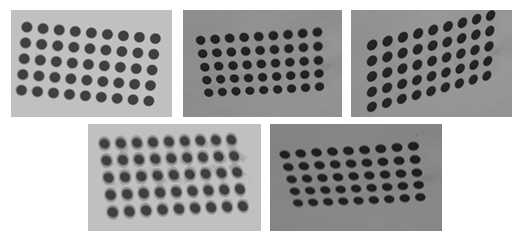
\includegraphics[height=4cm, width=8cm]{figures/eximg.png}
	\caption {Five examples of images captured by the camera under Scheimpflug set-up.}

	\label{fig:datagrid}
\end{figure}



The target is composed of circle grids rather than checkerboard so that the feature points can be well detected even when the images are blurred. The diameter of the circle pattern is 5 mm, the extracted feature points are the circle gravity centers  and the distance between two feature points is 7.5mm. 


\begin{table}[h!]
  \begin{center}
\begin{tabular}{l*{7}{c}r}
\hline
Parameter             & $f_x $ & $f_y $&  $u_0 $ & $v_0$  & $f$(mm)& $\theta(^{\circ})$ & Mean error & Standard Deviation \\
		Unit					&	(mm)& (mm) &   (px) &  (px) & (mm)& $(^{\circ})$ & 						(px)	&	(px)\\
\hline
Value            & 3717.3& 3716.0 & 517.5&587.8&24.9 & 1.49 & 0.15 & 0.037  \\
\hline
\end{tabular}
  \end{center}
  \caption{Calibration result from combined target.}
\label{tab:resuty112}
\end{table}

The feature extraction and  calibration procedure explained earlier provide the calibration results detailed in Table  \ref{tab:resuty112}. We have assessed the calibration performance by computing the mean and standard deviation of re-projection error over the 25 captured images. Scheimpflug angle has been well estimated and the mean error allows accurate 3D measures.

\section{Conclusion}

A new method for the calibration of cameras under Scheimpflug conditions has been presented. This method extends the pin-hole camera model where the image plane is perpendicular to the optical axis, by adding the Scheimpflug tilt angle $\theta$. To simplify distortion as a result of the tilted effect, we proposed to project the pixels on the tilted plane to the untilted ones using the proposed formation model. We assume that the tilt effect can be considered as large radial distortions, so we do not need to simplify the radial distortion parameters afterwards.  Then, we can extract camera parameters from the projected pixels on the untilted image plane using the same approach as Zhang et al. method \cite{Zhang:2000:FN}. Finally, a bundle adjustment approach based on Levenberg-Marquardt  is used to refine the intrinsic camera parameters.

\bibliographystyle{elsarticle-num}
%\bibliographystyle{elsarticle-harv}
\bibliography{myref}


%\section*{Formatting Citations}
%
%Citations can be handled in one of three ways.  The most
%straightforward (albeit labor-intensive) would be to hardwire your
%citations into your \LaTeX\ source, as you would if you were using an
%ordinary word processor.  Thus, your code might look something like
%this:
%
%
%\begin{quote}
%\begin{verbatim}
%However, this record of the solar nebula may have been
%partly erased by the complex history of the meteorite
%parent bodies, which includes collision-induced shock,
%thermal metamorphism, and aqueous alteration
%({\it 1, 2, 5--7\/}).
%\end{verbatim}
%\end{quote}
%
%
%\noindent Compiled, the last two lines of the code above, of course, would give notecalls in {\it Science\/} style:
%
%\begin{quote}
%\ldots thermal metamorphism, and aqueous alteration ({\it 1, 2, 5--7\/}).
%\end{quote}
%
%Under the same logic, the author could set up his or her reference list as a simple enumeration,
%
%\begin{quote}
%\begin{verbatim}
%{\bf References }
%
%\begin{enumerate}
%
%
%
%@article{Zhang:2000:FN,
% author = {Zhang, Zhengyou},
% title = {A Flexible New Technique for Camera Calibration},
% journal = {IEEE Trans. Pattern Anal. Mach. Intell.},
% issue_date = {November 2000},
% volume = {22},
% number = {11},
% month = nov,
% year = {2000},
% issn = {0162-8828},
% pages = {1330--1334},
% numpages = {5},
% url = {http://dx.doi.org/10.1109/34.888718},
% doi = {10.1109/34.888718},
% acmid = {357025},
% publisher = {IEEE Computer Society},
% address = {Washington, DC, USA},
% keywords = {Camera calibration, calibration from planes, 2D pattern, flexible plane-based calibration, absolute conic, projective mapping, lens distortion, closed-form solution, maximum likelihood estimation, flexible setup.},
%} 
%
%
%
%
%
%
%\end{enumerate}
%\end{verbatim}
%\end{quote}

%\noindent .\\

%\begin{quote}
%{\bf References }
%
%\begin{enumerate}
%\item Zhengyou Zhang, {\it A Flexible New Technique for Camera Calibration\/} (IEEE Trans. Pattern Anal. Mach. Intell., Pages 1330--1334, November, 2000).
%
%%\item G. Gamow, {\it The Constitution of Atomic Nuclei and
%%Radioactivity\/} (Oxford Univ. Press, New York, 1931).
%%\item W. Heisenberg and W. Pauli, {\it Zeitschr.\ f.\ Physik} {\bf 56},
%%1 (1929).
%\end{enumerate}
%\end{quote}

%That's not a solution that's likely to appeal to everyone, however ---
%especially not to users of B{\small{IB}}\TeX\ \cite{inclme}.  If you
%are a B{\small{IB}}\TeX\ user, we suggest that you use the
%\texttt{Science.bst} bibliography style file and the
%\texttt{scicite.sty} package, both of which we are downloadable from our author help site
%(http://www.sciencemag.org/about/authors/prep/TeX\_help/).  You can also
%generate your reference lists by using the list environment
%\texttt{\{thebibliography\}} at the end of your source document; here
%again, you may find the \texttt{scicite.sty} file useful.
%
%Whether you use B{\small{IB}}\TeX\ or \texttt{\{thebibliography\}}, be
%very careful about how you set up your in-text reference calls and
%notecalls.  In particular, observe the following requirements:
%
%\begin{enumerate}
%\item Please follow the style for references outlined at our author
%  help site and embodied in recent issues of {\it Science}.  Each
%  citation number should refer to a single reference; please do not
%  concatenate several references under a single number.
%\item Please cite your references and notes in text {\it only\/} using
%  the standard \LaTeX\ \verb+\cite+ command, not another command
%  driven by outside macros.
%\item Please separate multiple citations within a single \verb+\cite+
%  command using commas only; there should be {\it no space\/}
%  between reference keynames.  That is, if you are citing two
%  papers whose bibliography keys are \texttt{keyname1} and
%  \texttt{keyname2}, the in-text cite should read
%  \verb+\cite{keyname1,keyname2}+, {\it not\/}
%  \verb+\cite{keyname1, keyname2}+.
%\end{enumerate}
%
%\noindent Failure to follow these guidelines could lead
%to the omission of the references in an accepted paper when the source
%file is translated to Word via HTML.
%
%\section*{Handling Math, Tables, and Figures}
%
%Following are a few things to keep in mind in coding equations,
%tables, and figures for submission to {\it Science}.
%
%\paragraph*{In-line math.}  The utility that we use for converting
%from \LaTeX\ to HTML handles in-line math relatively well.  It is best
%to avoid using built-up fractions in in-line equations, and going for
%the more boring ``slash'' presentation whenever possible --- that is,
%for \verb+$a/b$+ (which comes out as $a/b$) rather than
%\verb+$\frac{a}{b}$+ (which compiles as $\frac{a}{b}$).  Likewise,
%HTML isn't tooled to handle certain overaccented special characters
%in-line; for $\hat{\alpha}$ (coded \verb+$\hat{\alpha}$+), for
%example, the HTML translation code will return [\^{}$(\alpha)$].
%Don't drive yourself crazy --- but if it's possible to avoid such
%constructs, please do so.  Please do not code arrays or matrices as
%in-line math; display them instead.  And please keep your coding as
%\TeX-y as possible --- avoid using specialized math macro packages
%like \texttt{amstex.sty}.
%
%\paragraph*{Displayed math.} Our HTML converter sets up \TeX\
%displayed equations using nested HTML tables.  That works well for an
%HTML presentation, but Word chokes when it comes across a nested
%table in an HTML file.  We surmount that problem by simply cutting the
%displayed equations out of the HTML before it's imported into Word,
%and then replacing them in the Word document using either images or
%equations generated by a Word equation editor.  Strictly speaking,
%this procedure doesn't bear on how you should prepare your manuscript
%--- although, for reasons best consigned to a note \cite{nattex}, we'd
%prefer that you use native \TeX\ commands within displayed-math
%environments, rather than \LaTeX\ sub-environments.
%
%\paragraph*{Tables.}  The HTML converter that we use seems to handle
%reasonably well simple tables generated using the \LaTeX\
%\texttt{\{tabular\}} environment.  For very complicated tables, you
%may want to consider generating them in a word processing program and
%including them as a separate file.
%
%\paragraph*{Figures.}  Figure callouts within the text should not be
%in the form of \LaTeX\ references, but should simply be typed in ---
%that is, \verb+(Fig. 1)+ rather than \verb+\ref{fig1}+.  For the
%figures themselves, treatment can differ depending on whether the
%manuscript is an initial submission or a final revision for acceptance
%and publication.  For an initial submission and review copy, you can
%use the \LaTeX\ \verb+{figure}+ environment and the
%\verb+\includegraphics+ command to include your PostScript figures at
%the end of the compiled PostScript file.  For the final revision,
%however, the \verb+{figure}+ environment should {\it not\/} be used;
%instead, the figure captions themselves should be typed in as regular
%text at the end of the source file (an example is included here), and
%the figures should be uploaded separately according to the Art
%Department's instructions.
%
%
%\section*{What to Send In}
%
%What you should send to {\it Science\/} will depend on the stage your manuscript is in:
%
%\begin{itemize}
%\item {\bf Important:} If you're sending in the initial submission of
%  your manuscript (that is, the copy for evaluation and peer review),
%  please send in {\it only\/} a PostScript or PDF version of the
%  compiled file (including figures).  Please do not send in the \TeX\ 
%  source, \texttt{.sty}, \texttt{.bbl}, or other associated files with
%  your initial submission.  (For more information, please see the
%  instructions at our Web submission site,
%  http://www.submit2science.org/ .)
%\item When the time comes for you to send in your revised final
%  manuscript (i.e., after peer review), we require that you include
%  all source files and generated files in your upload.  Thus, if the
%  name of your main source document is \texttt{ltxfile.tex}, you
%  need to include:
%\begin{itemize}
%\item \texttt{ltxfile.tex}.
%\item \texttt{ltxfile.aux}, the auxilliary file generated by the
%  compilation.
%\item A PostScript file (compiled using \texttt{dvips} or some other
%  driver) of the \texttt{.dvi} file generated from
%  \texttt{ltxfile.tex}, or a PDF file distilled from that
%  PostScript.  You do not need to include the actual \texttt{.dvi}
%  file in your upload.
%\item From B{\small{IB}}\TeX\ users, your bibliography (\texttt{.bib})
%  file, {\it and\/} the generated file \texttt{ltxfile.bbl} created
%  when you run B{\small{IB}}\TeX.
%\item Any additional \texttt{.sty} and \texttt{.bst} files called by
%  the source code (though, for reasons noted earlier, we {\it
%    strongly\/} discourage the use of such files beyond those
%  mentioned in this document).
%\end{itemize}
%\end{itemize}
%
%% Your references go at the end of the main text, and before the
%% figures.  For this document we've used BibTeX, the .bib file
%% scibib.bib, and the .bst file Science.bst.  The package scicite.sty
%% was included to format the reference numbers according to *Science*
%% style.
%%
%%   this is for BibTeX.  remove if you plan to write the references in the document
%\bibliographystyle{plain}
%\bibliography{mybiblio}
%
%%
%%
%
%
%
%% Following is a new environment, {scilastnote}, that's defined in the
%% preamble and that allows authors to add a reference at the end of the
%% list that's not signaled in the text; such references are used in
%% *Science* for acknowledgments of funding, help, etc.
%
%\begin{scilastnote}
%\item We've included in the template file \texttt{scifile.tex} a new
%environment, \texttt{\{scilastnote\}}, that generates a numbered final
%citation without a corresponding signal in the text.  This environment
%can be used to generate a final numbered reference containing
%acknowledgments, sources of funding, and the like, per {\it Science\/}
%style.
%\end{scilastnote}




% For your review copy (i.e., the file you initially send in for
% evaluation), you can use the {figure} environment and the
% \includegraphics command to stream your figures into the text, placing
% all figures at the end.  For the final, revised manuscript for
% acceptance and production, however, PostScript or other graphics
% should not be streamed into your compliled file.  Instead, set
% captions as simple paragraphs (with a \noindent tag), setting them
% off from the rest of the text with a \clearpage as shown  below, and
% submit figures as separate files according to the Art Department's
% instructions.


%\clearpage
%
%\noindent {\bf Fig. 1.} Please do not use figure environments to set
%up your figures in the final (post-peer-review) draft, do not include graphics in your
%source code, and do not cite figures in the text using \LaTeX\
%\verb+\ref+ commands.  Instead, simply refer to the figure numbers in
%the text per {\it Science\/} style, and include the list of captions at
%the end of the document, coded as ordinary paragraphs as shown in the
%\texttt{scifile.tex} template file.  Your actual figure files should
%be submitted separately.



\end{document}




















